
%%%%%%%%%%%%%
%     BACKGROUND     %
%%%%%%%%%%%%%

\begin{figure}
\centering
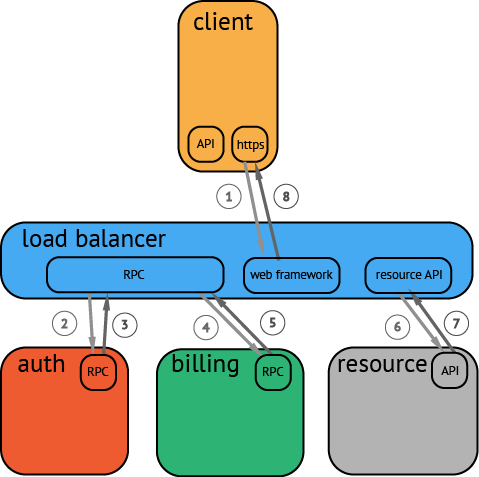
\includegraphics[width=\textwidth,height=6cm,keepaspectratio=true]{basic_trace}
\caption{A sample trace}
\label{basic_trace}
\end{figure}

\begin{figure}
\centering
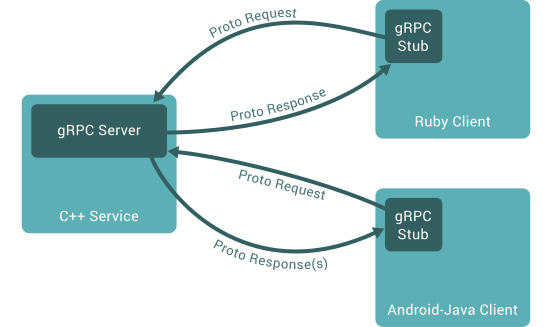
\includegraphics[width=8cm,height=6cm,keepaspectratio=true]{grpc_arch}
\caption{Architecture of gRPC}
\label{grpc_arch}
\end{figure}


\section{Background and Motivation}
This section will provide an overview of Opentracing, the 
types of wire protocols that we explore for cross-process communication
and how annotations are propagated through them, and the reasoning behind 
integrating the fault injection mechanism into the tracing framework. \kmd{need a proper intro}

%%%%%%%%%%%%%%
%     OPEN TRACING     %
%%%%%%%%%%%%%%
\subsection{OpenTracing}
Today's microservice architectures are large in scale and highly complex and often consist 
of services written many languages. The characteristics render the process of developing a principled and useful distributed tracing framework over these services
extremely challenging. Opentracing\cite{opentracing:doc} provides a set of vendor-neutral
APIs for obtaining distributed traces through annotation propagation and allows for easy
integration into existing microservice architectures. Previously available solutions for tracing through
application level annotations such as Magpie\cite{magpie} and X-Trace\cite{xtrace} are unappealing
because of the per-application schema requirement exacerbates the level of integration inconvenience and introduces higher application overheads \cite{sigelman:dapper}. For these reasons,
we chose to use the Opentracing APIs to provide our architecture with fine-grained traces. 


%%%%%%%%%%%%%%%%%%%
%     TRACE TERMINOLOGIES     %
%%%%%%%%%%%%%%%%%%%
\subsubsection{Trace Terminologies}
A \textbf{span} is a basic, logical unit of work with a start time and duration and exists within 
a single service. Spans can be nested to show causal relation. \textbf{Baggage} is a set of \textless K,V\textgreater pairs wrapped within a span's context and allows for transparent propagation of arbitrary data. A \textbf{tracer} consists of a set of spans belonging to a group of services. For example, a set of REST endpoints belonging to a group of services in a server manifests a tracer. For cross-process tracing, a tracer will \textbf{inject} the span's context, and \textbf{extract} it on the other end. \kmd{definitions of inject/extract?}


%%%%%%%%%%%%
%     TRACE FLOW     %
%%%%%%%%%%%%
\subsubsection{Trace flow}
Each service that a developer wishes to be traced will need to have a span constructed, after which it
will be added to a list of spans in the global tracer. Each span will automatically provide trace detail consisting of a timestamp and duration; the developer can decorate the span with more details, such as the status of a lock or value of a variable by adding to the span's baggage. When a service calls another service,
the tracer will have to be invoked to inject the local span's context into the wire, and extracted on the other side. During the extraction, a new(child) span is constructed from old(parent) span's context. Spans are recorded in the order that they are finished, meaning that whichever finishes first will be first to output trace information to the output stream. Figure \ref{basic_trace} shows a simple trace involving several microservices\cite{opentracing:doc}.


%%%%%%%%%%%%%%%
%     FAULT HANDLING     %
%%%%%%%%%%%%%%%
\subsection{Fault Handling}
There are three ways one could approach adding a fault injection component into a microservice architecture. The first approach consists of incorporating the FI component into the constituent services of the microservice architecture individually. Each service will have a special chunk of code capable of reacting to fault injection information received from upstream. \kmd{what kind of reactions?} The obvious advantage of the approach is the ease of implementation. Additionally, the developer exerts full control on how each service should react to a type of failure. However, the approach requires the existence of FI code in all target services. Such a task is intractable if particular microservice architectures contain hundreds of services written in a multitude of languages \kmd{example(s)?}.

The second approach places the onus of fault handling upon the wire protocol. If all services communicate through a single protocol (e.g. HTTP), then the method greatly reduces the absolute amount of code required to support and manage fault triggers. Accordingly, even if subsets of services use different protocols, the amount of code devoted to FI support is proportional to the number of different communication protocols, which should be in the single digits. The downside of the approach is the need to extend the bare communication protocol, which may necessitate modifying hardened core components in a process very vulnerable to the possibility of introducing new bugs capable of violating the integrity of the communication protocol.

The third approach, which represents the core philosophy behind RLFI, advocates the incorporation of fault handling mechanisms at the programming language level. \kmd{what do you mean by programming language level? need a paragraph description.} The method is practical from an implementation perspective because the number of languages in a service is bounded between ten and twenty \kmd{citation?}. The approach also avoids the risk of polluting both the underlying application code and the code for the chosen wire protocol(s). As an example, to incorporate a FI framework over a set of HTTP REST endpoints written in golang\cite{google:golang}, the only necessary changes are wrapping the communication protocol handler functions inside decorators. Below is a code listing of how one would implement this: \kmd{make this a figure}


\begin{lstlisting}[basicstyle=\tiny, ] %or \small or \footnotesize etc.

func homeHandler(w http.ResponseWriter, r *http.Request) {
    //stuff goes here
}

func decorate(f http.HandlerFunc) http.HandlerFunc {
    return func(w http.ResponseWriter, r *http.Request) {
        //do some preprocessing of the request
        f(w, r) //call the function
    }
}

func main() {
    http.HandleFunc("/home", decorate(homeHandler))

    http.ListenAndServe("localhost:8080", nil)
}
\end{lstlisting}

Notice that the changes to the application are minor and the decorator has full access to whatever was passed over the wire.


%%%%%%%%%%%%%%%
%     WIRE PROTOCOLS     %
%%%%%%%%%%%%%%%
\subsection{Wire Protocols}
Wire protocols are used for writing application-level code for cross-process communication. 
Protocols such as HTTP, gRPC\cite{google:grpc}, and Thrift\cite{apache:thrift} support the sending and receipt of data between services within mircroservice architectures. Opentracing supports both HTTP and gRPC as wire protocols and uses both to support the propagation of span context between particular, but arbitrary, services throughout the system. In gRPC, clients expose methods called remotely from servers to support client call management. Data passes along gRPC wires in the 
form of Protocol Buffers\cite{google:protobuf}. Figure \ref{grpc_arch} illustrates the basic flow of the gRPC architecture\cite{google:grpc}.


%%%%%%%%%%%%
%     MOTIVATION     %
%%%%%%%%%%%%
\subsection{Motivation}
We believe fine-grained traces and request-level fault injection are complementary.
One of the primary motivations for obtaining traces of large-scale distributed services is to support analyzes of results derived from 
bad executions to identify weak points capable of preventing appropriate responses to client requests. Such  weak points 
represent ideal targets for fault injections in experiments verifying failure scenarios.
We would like to take advantage of Opentracing's built-in mechanisms for easily passing arbitrary baggage between services to propagate request-level faults through baggage items. 

%Of course, one could propagate such requests through the wire protocols themselves, bypassing the overhead of constructing spans and injecting them. However, the overhead associated with implementation and fault injection are extremely small because Opentracing's APIs allow for a clean way of handling the baggage data. 


%%%%%%%
%    EOF     %
%%%%%%%